\section{How Good is Our Prediction?}
\label{sec:theorems}

We have built machines that \textit{seem} to capture the structure of a process. We calculated their complexity and entropy. But how do we know if they are actually \textit{good} models?

Shalizi and Crutchfield (2001) give us two powerful guarantees---two "Fundamental Theorems" of Computational Mechanics.

\subsection{Theorem 1: Prescience (Accuracy)}

The first question is simple: \textbf{Does our model predict the future as well as the past allows?}

Imagine an Oracle who remembers the \textit{entire} infinite history of the universe ($\overleftarrow{X}$). We, on the other hand, only know the current causal state ($\mathcal{S}$).
Theorem 1 states that valid causal states are \textbf{prescient}:
\[ P(\vec{X} | \mathcal{S}) = P(\vec{X} | \overleftarrow{X}) \]
In English: \textit{Knowing the causal state is just as good as knowing the entire history.} You lose zero predictive power by compressing the history into a state.

\begin{intuition}
    \textbf{The Cost of Being Wrong: KL Divergence}\\
    To measure how wrong a model is, we use the \textbf{Kullback-Leibler (KL) Divergence}. Think of it as a "distance" between two probability distributions.

    If the true distribution of future symbols is $P$ and our model predicts $Q$, the KL divergence $D_{KL}(P || Q)$ tells us how many extra bits we need to correct our mistake.
    \begin{itemize}
        \item If $D_{KL} = 0$, our model is perfect.
        \item If $D_{KL} > 0$, our model is missing something.
    \end{itemize}
\end{intuition}

We can verify this theorem numerically. In \texttt{emic}, we can sweep through different complexity levels (by adjusting the significance level $\alpha$ of the statistical test) and measure the error.

\begin{emiclisting}[label=lst:optimality]{Checking Optimality}
\begin{lstlisting}[language=Python, basicstyle=\tiny\ttfamily, numbers=none]
# Does adding more states reduce error?
results = []
for alpha in [0.001, 0.01, 0.1, 0.5]:
    # Infer machine with decreasing strictness
    machine = cssr.infer(data, alpha)
    # Measure complexity (C_mu) and error (excess entropy)
    results.append((machine.c_mu, machine.kl_divergence))
\end{lstlisting}
\end{emiclisting}

In Figure \ref{fig:optimality}, we plot the prediction error (KL Divergence) against the number of states.

\begin{emicfigure}[label=fig:optimality]{The Optimality Curve}
    \centering
    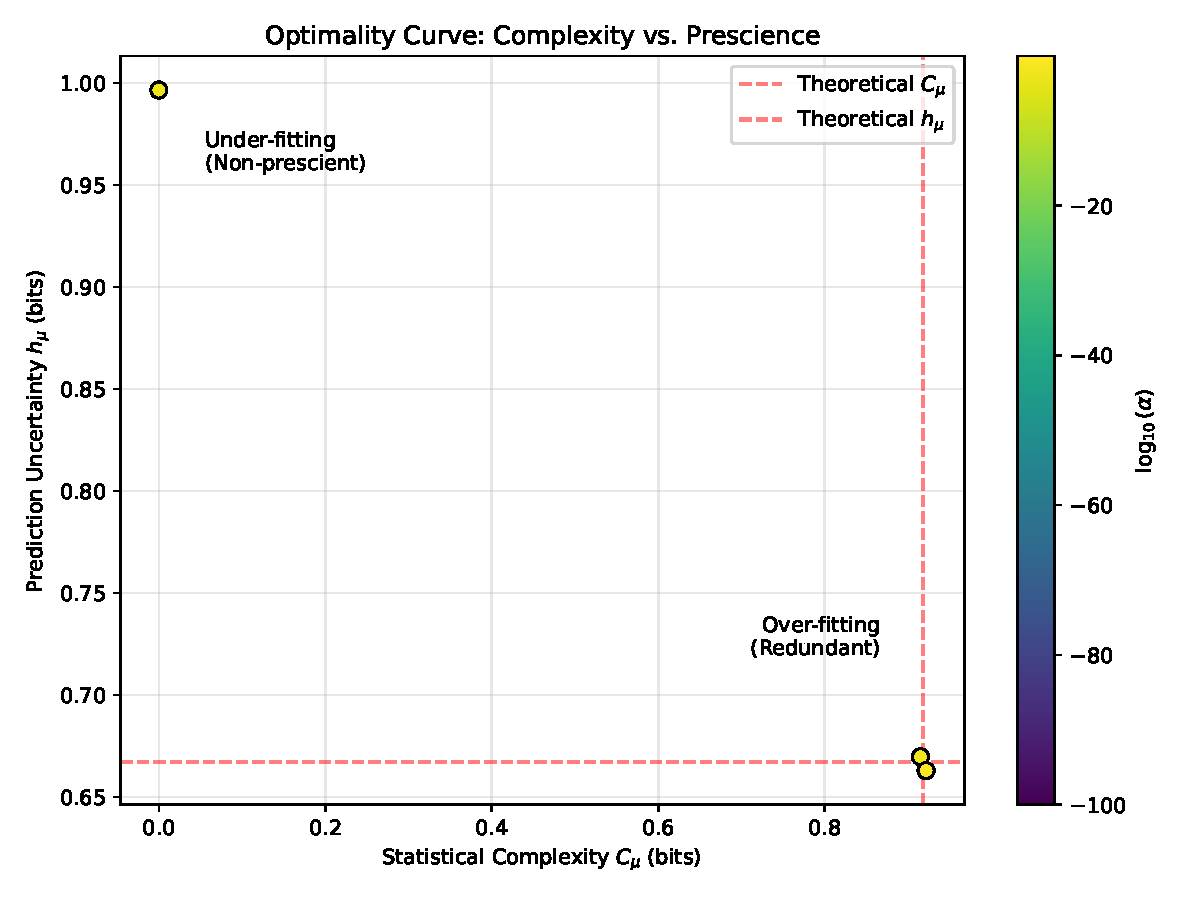
\includegraphics[width=\columnwidth]{figures/optimality_curve.pdf}

    The x-axis is complexity (number of states), the y-axis is prediction error ($D_{KL}$). The $\epsilon$-machine sits at the "elbow": minimal complexity for zero error.
\end{emicfigure}

Notice the curve. As we add more states (moving to the right), the error drops. But once we hit the "correct" number of states (the $\epsilon$-machine), the error hits zero. Adding more states after that point doesn't help---it just wastes memory.

\subsection{Theorem 2: Minimality (Efficiency)}

The second question is about efficiency: \textbf{Is this the smallest possible correct model?}

You could predict the future perfectly by simply memorizing every sequence of length 1000. That would be "prescient" (zero error), but it would be huge ($2^{1000}$ states!).

Theorem 2 states that among all prescient models, the $\epsilon$-machine is the \textbf{minimal} one. It has the smallest possible statistical complexity ($C_\mu$).
\[ C_\mu(\epsilon\text{-machine}) \leq C_\mu(\text{any other prescient model}) \]

This confirms that the $\epsilon$-machine is the \textbf{unique, simplest, optimal predictor} of a process.
